\documentclass[11pt]{article}
\usepackage[a4paper,landscape,margin=0.72in]{geometry}
\usepackage[T1]{fontenc}
\usepackage{lmodern,amsmath,amssymb,graphicx,hyperref}
\title{Derivative-point case: an actual weighted-Proj DVR}
\author{Formal proof packet}
\date{28 October 2026}
\begin{document}
\maketitle
\noindent This packet records a checked local geometry theorem. It contains no experiment, target result, or cost ratio. The Lean source, compiler log, editable SVG, and CSV gate table accompany this PDF.

\section*{Checked boundary}
Let $K$ be any field, $f(X)=X^5+a_3X^3+a_2X^2+a_1X+a_0$, and $(a,y)\in K^2$ satisfy $y^2=f(a)$. Assume $f$ is separable and $f'(a)\ne0$. The difference quotient $q_a(X)=(f(X)-f(a))/(X-a)$ has $q_a(a)=f'(a)$, so it is a unit in the local ring at $(a,y)$. The checked point ideal is $(X-a,Y-y)$, and the curve relation gives
\[
  (Y-y)(Y+y)=(X-a)q_a(X).
\]
Hence the local maximal ideal is generated by $Y-y$. Its generator is nonzero. Separability supplies the coordinate-ring domain, and the checked DVR criterion makes the affine localization a discrete valuation ring. The checked ring equivalence transfers this structure to the \emph{actual weighted-$\operatorname{Proj}$ point stalk}. The theorem works in characteristic two when this pointwise derivative condition holds; it does not assume $2y\ne0$.

\section*{Scope and verification}
No DVR claim is made when both partial derivatives vanish. Over $\mathbf F_2$, $f=X^5+X^3+1$ is separable but $(0,1)$ is singular. A combined theorem for the two pointwise smoothness cases remains open in this formal line.

Direct pinned Lean 4.34.1 compilation exited zero against Mathlib revision
\par\noindent\texttt{d13f23b723b8a846827a245b89c10fc7d3f11612}.
Five printed axiom audits list only \texttt{propext}, \texttt{Classical.choice}, and \texttt{Quot.sound}; no \texttt{sorryAx}. Source SHA-256:
\par\noindent{\small\texttt{0e9a8e7a31ab5dc8564b13611683989880dee03428be5e4b9e690fac6d969197}}.
The compiler log retains nonfatal style-linter suggestions. The local DVR criterion follows pinned Mathlib \texttt{IsDiscreteValuationRing.TFAE} and Stacks Project Tag 00PD. The prior checked stalk equivalence uses the open-immersion principle of Stacks Tag 01HD.

Formula-specific common 2+2 norm transport, global principal-divisor/$\mathrm{Pic}^0$ transport, and compiled Rust semantics remain open. The CSV records exact gate statuses.

\clearpage
\section*{Proof dependencies and open gates}
\begin{center}
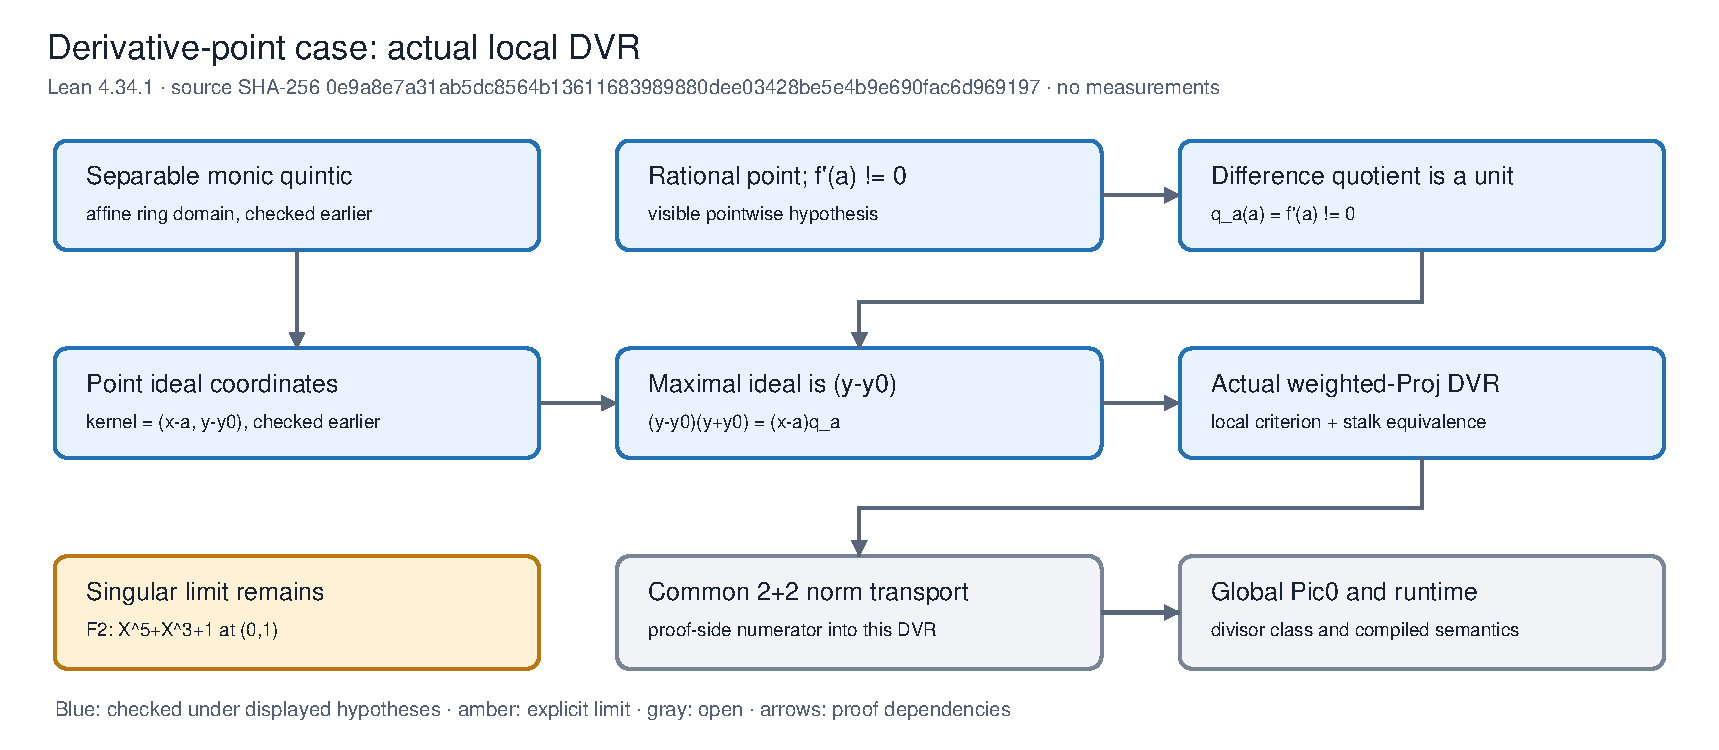
\includegraphics[width=0.96\textwidth,height=0.76\textheight,keepaspectratio]{derivative-point-dvr-figure.pdf}
\end{center}
\noindent Blue nodes are checked under the displayed hypotheses. Amber records the singular limit; gray nodes are open. Arrows show proof dependencies, not measured performance.
\end{document}
